% !TEX root =  ../main_manuscript.tex 
\section{Introduction}
Patients with low- and very low-risk screening-detected localized prostate cancer are usually advised active surveillance (AS) instead of immediate radical treatment \citep{briganti2018active}. In AS, cancer progression is routinely monitored via prostate-specific antigen (PSA), digital rectal examination, and repeat biopsies. Among these, biopsy Gleason grade is the strongest indicator of cancer-related outcomes \citep{epsteinGG2014}. When the Gleason grade increases from grade~1 [Gleason score $\leq$ 6 (3+3)] to grade~2 [Gleason score 7 (3+4)] or higher (reclassification), the patient is commonly advised curative treatment \citep{bul2013active}.

Biopsies are conducted periodically, and hence reclassification is always detected with a time delay (Figure~\ref{fig:delay_explanation}). The smaller this time delay, the larger is the window of opportunity for curative treatment. For detecting reclassification timely, many AS programs use fixed and frequent biopsy schedules (e.g., annual biopsies) for all patients \citep{nieboer2018active,loeb2014heterogeneity}. However, such schedules also lead to many unnecessary biopsies in slow/non-progressing patients. Biopsies are invasive, painful and prone to medical complications. Thus, biopsy burden combined with patient non-compliance to frequent biopsies \citep{bokhorst2015compliance} has raised concerns regarding the optimal biopsy schedule \citep{inoue2018comparative, bratt2013study}.

\begin{figure}
\centerline{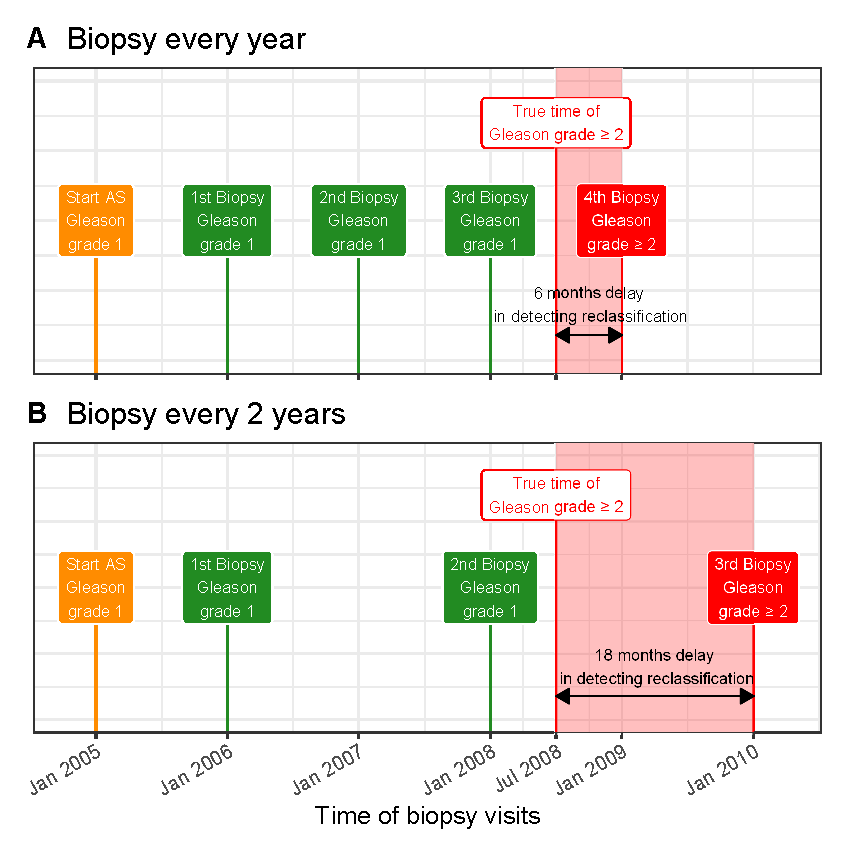
\includegraphics[width=\columnwidth]{images/delay_explanation.eps}}
\caption{\textbf{Trade-off between the number of biopsies and time delay in detecting reclassification (Increase in Gleason grade from 1 to 2):} The true time of reclassification for the patient in this figure is July 2008. When biopsies are scheduled annually (\textbf{Panel~A}), reclassification is detected in January 2009 with a time delay of six months, and a total of four biopsies are scheduled. When biopsies are scheduled biennially (\textbf{Panel~B}) reclassification is detected in January 2010 with a time delay of 18 months, and a total of three biopsies are scheduled. Since biopsies are conducted periodically, the time of reclassification is observed as an interval. For example, Jan~2008--Jan~2009 in \textbf{Panel~A} and Jan~2008--Jan~2010 in \textbf{Panel~B}.}
\label{fig:delay_explanation}
\end{figure}

%\begin{figure}[!htb]
%\centerline{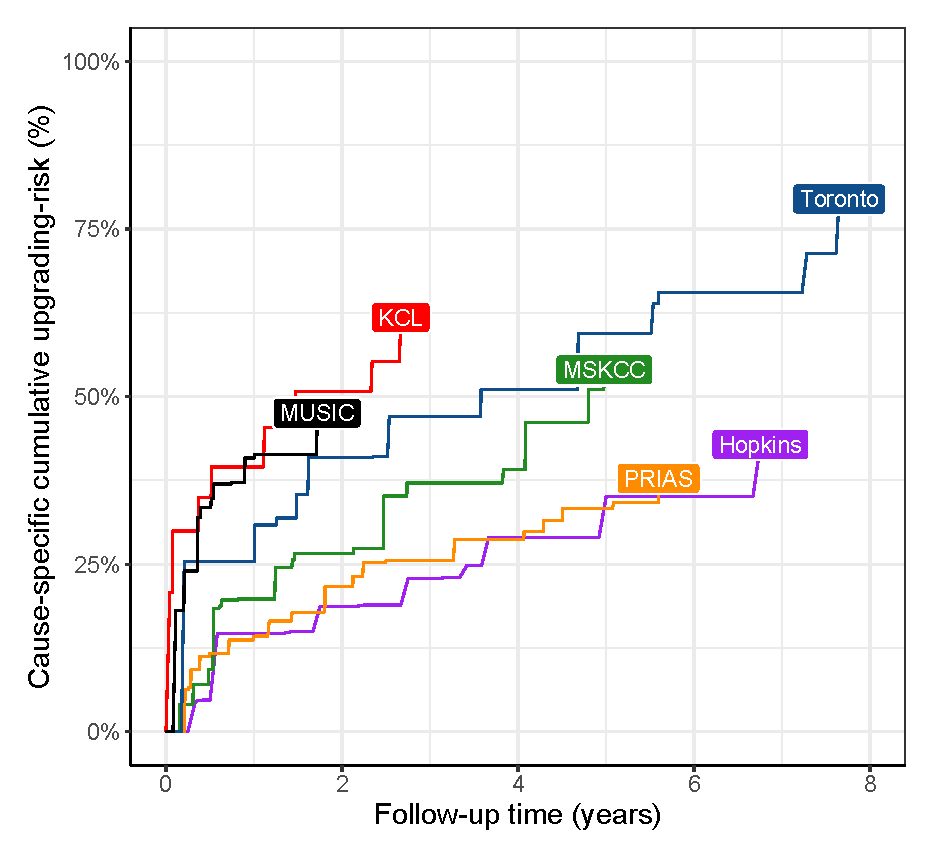
\includegraphics[width=\columnwidth]{images/npmle_plot.eps}}
%\caption{\textbf{Estimated cumulative risk of having Gleason~$\geq$~7 (reclassification)} in the world's largest AS cohort PRIAS, and five of the largest AS cohorts part of the GAP3 database \citep{gap3_2018}. Abbreviations are \textit{JHAS}: Johns Hopkins Active Surveillance, \textit{PRIAS}: Prostate Cancer International Active Surveillance, \textit{Toronto}: University of Toronto Active Surveillance, \textit{MSKCC}: Memorial Sloan Kettering Cancer Center Active Surveillance, \textit{KCL}: King's College London Active Surveillance. In the world's largest AS cohort PRIAS and in JHAS, roughly 50\% of patients do not obtain reclassification in the first ten years. That is, ideally, no biopsies should be prescribed to 50\% of the patients in the first ten years of AS.}
%\label{fig:npmle_plot}
%\end{figure}

A simple alternative to fixed and frequent biopsies is infrequent biopsies. For example, scheduling biopsies biennially instead of annually, may not substantially increase the risk of adverse downstream outcomes \citep{inoue2018comparative,de2017estimating}. Although, scheduling biopsies biennially may still lead to five unnecessary biopsies over ten years (current study period of large AS programs) for slow/non-progressing patients. A promising alternative to fixed biopsies is personalized schedule of biopsies. Personalized schedules utilize a patient's risk of reclassification to make decisions for biopsies (Figure~\ref{fig:riskBasedExample}).

\begin{figure}
\centerline{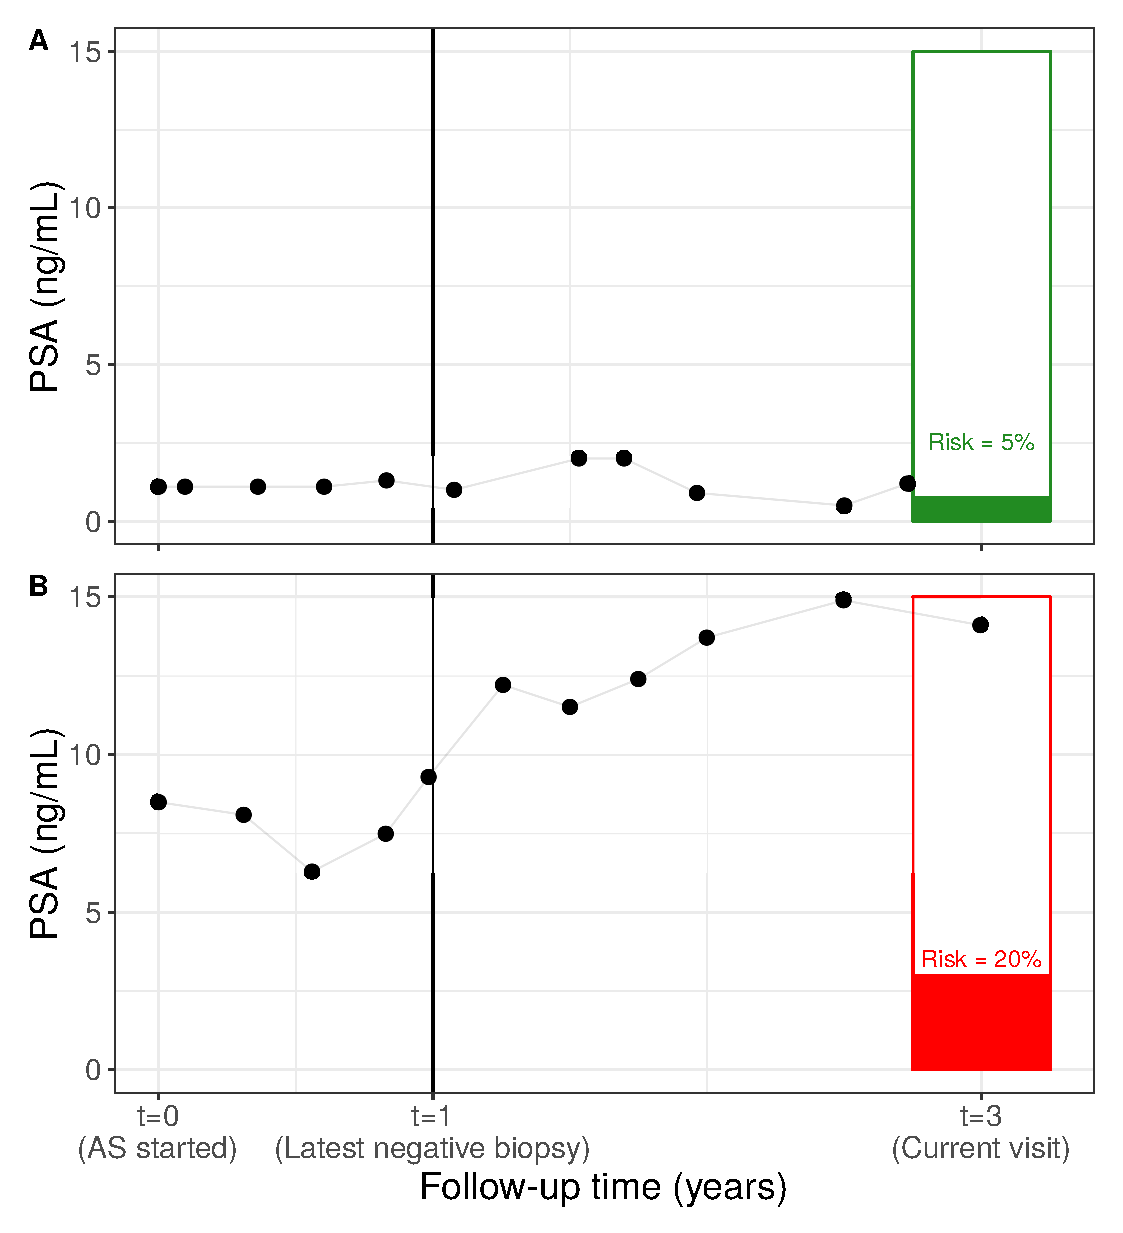
\includegraphics[width=\columnwidth]{images/riskBasedExample.eps}}
\caption{\textbf{Motivation for personalized risk-based decisions of biopsy}: Patients A (\textbf{Panel~A}) and B (\textbf{Panel~B}) had their latest biopsy at year one of follow-up (green vertical line). Patient A's prostate-specific antigen profile remained stable until his current visit at year three, whereas patient B's profile has shown a rise. Consequently, patient B's estimated cumulative risk of reclassification at the current visit (year three) is higher than that of patient A. This makes patient B a more suitable candidate for biopsy than Patient A. \textit{Risk estimates in this figure are only illustrative.}}
\label{fig:riskBasedExample}
\end{figure}

The first challenge in developing risk of reclassification based personalized schedules is consolidating observed patient data (e.g., PSA, previous biopsy results) into risk estimates for reclassification. Previous studies have utilized the latest value of PSA to predict the Gleason grade \citep{partin1993use,makarov2007updated}. However, this approach ignores historical PSA measurements. To combine such longitudinal PSA data with historical biopsy results, a suitable model is the joint model for time-to-event and longitudinal data \citep{tomer2019,coley2017prediction,rizopoulos2012joint}. This model provides personalized predictions for risk of reclassification. Although, the subsequent challenge is to translate risk predictions into clinical decisions. For example, a 10\% risk of reclassification can be perceived as high/low depending upon the patient's age. Patients may also weigh these risks with the potential \textit{consequences} of another biopsy. Two relevant \textit{consequences} of biopsies (Figure~\ref{fig:delay_explanation}) are the timing and total number of biopsies (burden), and the time delay in detecting reclassification (smaller is beneficial). The relative importance of these \textit{consequences} can vary between the patients, and also over the follow-up period for the same patient.

The goal of this work was to assist patients and doctors in making better decisions of biopsies than fixed and frequent biopsies. For this purpose, we created a tool that provides patients their current and future risk of having a reclassification, and personalized schedules of biopsies based on these risks. The tool also provides expected \textit{consequences} of both fixed and personalized schedules. Thus, patients can compare them before making a decision. We took three steps for our goal. First, we fitted a prediction (joint) model to the world's largest AS dataset, PRIAS \citep{bul2013active}. We then externally validated it in five largest AS cohorts from the GAP3 database \citep{gap3_2018}. Lastly, we utilized our model to develop personalized schedule of biopsies, and to estimate the \textit{consequences} of following both personalized and fixed biopsy schedules.